\documentclass{article}


\usepackage[margin=1in]{geometry}
\usepackage{mathtools} %also loads amsmath
\usepackage{amssymb, bbm}
\usepackage[backend=biber,
	style=alphabetic,
	%	citestyle=authoryear,
	natbib=true,
	url=true, 
	doi=true]{biblatex}

%\usepackage{blkarray} % for matrices with labels
\usepackage{microtype}
\usepackage{relsize}
\usepackage{environ}% http://ctan.org/pkg/environ; for capturing body as a parameter for idxmats
\usepackage{tikz}
	\usetikzlibrary{positioning,fit,calc, decorations, arrows, shapes, shapes.geometric}
	\pgfdeclaredecoration{arrows}{draw}{
		\state{draw}[width=\pgfdecoratedinputsegmentlength]{%
			\path [every arrow subpath/.try] \pgfextra{%
				\pgfpathmoveto{\pgfpointdecoratedinputsegmentfirst}%
				\pgfpathlineto{\pgfpointdecoratedinputsegmentlast}%
			};
	}}
	%%%%%%%%%%%%
	
	\tikzset{dpadded/.style={rounded corners=2, inner sep=0.9em, draw, outer sep=0.4em, fill=gray, fill opacity=0.08, text opacity=1}}
	\tikzset{active/.style={fill=blue, fill opacity=0.1}}
	\tikzset{square/.style={regular polygon,regular polygon sides=4, rounded corners = 0}}
	\tikzset{octagon/.style={regular polygon,regular polygon sides=8, rounded corners = 0}}
	
	
	\tikzset{alternative/.style args={#1|#2|#3}{name=#1, circle, fill, inner sep=1pt,label={[name={lab-#1},gray!30!black]#3:\scriptsize #2}} }
	
	
	\tikzset{bpt/.style args={#1|#2}{alternative={#1|#2|above}} }
	\tikzset{tpt/.style args={#1|#2}{alternative={#1|#2|below}} }
	\tikzset{pt/.style args={#1}{alternative={#1|#1|above}} }
	

	\tikzset{mpt/.style args={#1|#2}{name=#1, circle, fill, inner sep=1pt,label={[name={lab-#1},gray]\scriptsize #2}} }
	\tikzset{pt/.style args={#1}{name=#1, circle, fill, inner sep=1pt,label={[name={lab-#1},gray]\scriptsize #1}} }
	
		
		 %\foreach \x in {#1}{(\x) (lab-\x) } 
		 
	\tikzset{Dom/.style args={#1 (#2) around #3}{dpadded, name=#2, label={[name={lab-#2}] #1}, fit={ #3 } }}
	\tikzset{Dom/.style args={#1 (#2) around #3}{dpadded, name=#2, label={[name={lab-#2}] #1}, fit={ #3 } }}
	\tikzset{bDom/.style args={#1 (#2) around #3}{dpadded, name=#2, label={[name={lab-#2}]below:#1}, fit={ #3 } }}
	\tikzset{arr/.style={draw, ->, thick, shorten <=3pt, shorten >=3pt}}
	\tikzset{archain/.style args={#1}{arr, every arrow subpath/.style={draw,arr, #1}, decoration=arrows, decorate}}
	%\tikzset{every label/.append style={text=red, font=\scriptsize}}
	
%	\newcommand\tikzdom[#1;#2](#3,#4[#5]){
%		\foreach [evaluate=\x as \y using (\x-#2/2)/#5 + #3] \x in {0, 1, ..., #2} {
%			\node[bpt={#1\x | $\n_\x$}] at (\y,#4) {};
%		}
%		\node[Dom={$\sf W$ (W) around \lab{w1}\lab{w3}}] {};
%	}

\usepackage{color}
\definecolor{deepgreen}{rgb}{0,0.5,0}

\usepackage[colorlinks=true, citecolor=deepgreen]{hyperref}


\setlength{\skip\footins}{1cm}
\setlength{\footnotesep}{0.4cm}

\usepackage{parskip}
\usepackage{amsthm, thmtools}
\usepackage{
	nameref,%\nameref
	hyperref,%\autoref
	% n.b. \Autoref is defined by thmtools
	cleveref,% \cref
	% n.b. cleveref after! hyperref
}

\begingroup
\makeatletter
\@for\theoremstyle:=definition,remark,plain\do{%
	\expandafter\g@addto@macro\csname th@\theoremstyle\endcsname{%
		\addtolength\thm@preskip\parskip
	}%
}
\endgroup
\makeatother

\theoremstyle{plain}
\newtheorem{theorem}{Theorem}[section]
\newtheorem{coro}{Corollary}[theorem]
\newtheorem{prop}[theorem]{Proposition}
\newtheorem{lemma}[theorem]{Lemma}
\newtheorem{fact}[theorem]{Fact}
\newtheorem{conj}[theorem]{Conjecture}

\theoremstyle{definition}
\newtheorem{defn}{Definition}[section]
\newtheorem{examplex}{Example}[section]
\newenvironment{example}
	{\pushQED{\qed}\renewcommand{\qedsymbol}{$\triangle$}\examplex}
	{\popQED\endexamplex\vspace{-1em}\rule{1cm}{0.7pt}\vspace{0.5em}}

\theoremstyle{remark}
\newtheorem*{remark}{Remark}

\usepackage{xstring}
\usepackage{enumitem}

%\newcommand\duplicat[1]{\gdef\mylist{}\foreach \x in {#1}{\xdef\mylist{\mylist (\x) (lab-\x) }}\mylist} %% this doesn't work :((
\newcommand\lab[1]{(#1)(lab-#1)}


\newcommand{\todo}[1]{{\color{red}\large\textbf{[todo}: {\normalsize\itshape#1}\textbf{]}}}
\newcommand\geqc{\succcurlyeq}
\newcommand\leqc{\preccurlyeq}
\newcommand\mat[1]{\mathbf #1}
\newcommand{\indi}[1]{\mathbbm{1}_{\left[\vphantom{\big[}#1 \vphantom{\big]}\right]}}
\newcommand\m[1]{\mathbf m_{\mathsf #1}}

\newcommand\recall[1]{ Recall \expandarg\cref{rex:#1}:\vspace{-1em} \begingroup\small\color{gray!80!black}\begin{quotation} \expandafter\csname rex:#1\endcsname* \end{quotation}\endgroup }

%OMG THIS WORKS

\def\wrapwith#1[#2;#3]{
	\expandafter#2{\expandarg\StrBefore{#1}{,}}
	\expandarg\StrBehind{#1}{,}[\tmp] 
	\xdef\tmp{\expandafter\unexpanded\expandafter{\tmp}}
	#3
	\expandarg\IfSubStr{\tmp}{,}{\wrapwith{\tmp}[#2;{#3}]}{ \expandafter#2{\tmp} }
}
\def\hwrapcells#1[#2]{\wrapwith#1[#2;&]}
\def\vwrapcells#1[#2]{\wrapwith#1[#2;\\]}



\newsavebox{\idxmatsavebox}
\def\makeinvisibleidxstyle#1#2{\phantom{\hbox{#1#2}}}
\newenvironment{idxmat}[3][\footnotesize\color{gray}\text]{%
	\def\idxstyle{#1}
	\def\colitems{#3}
	\def\rowitems{#2}
	\begin{lrbox}{\idxmatsavebox}$
	\begin{matrix}  \begin{matrix} \hwrapcells{\colitems}[\idxstyle]  \end{matrix} \\[0.1em]
		\left[ 
		\begin{matrix}
			\hwrapcells{\colitems}[\expandafter\makeinvisibleidxstyle\idxstyle]  \\[-1em]
	}{
		\end{matrix}\right]		&\hspace{-0.5em}\begin{matrix*}[l] \vwrapcells{\rowitems}[\idxstyle] \end{matrix*}
	\end{matrix}
	$\end{lrbox}
	\raisebox{0.75em}{\usebox\idxmatsavebox}
%	\vspace{-0.5em}
}

\newenvironment{sqidxmat}[2][\footnotesize\color{gray}\text]
	{\begingroup\idxmat[#1]{#2}{#2}}
	{\endidxmat\endgroup}
\usetikzlibrary{cd}

\usepackage{ wasysym }


\addbibresource{../refs.bib}
\addbibresource{../maths.bib}


\newcommand{\mfem}{\mathclap\female\male}
\newsavebox{\hourglassbox}
\savebox{\hourglassbox}{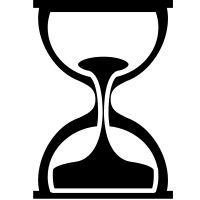
\includegraphics[height=.8em]{hourglass.png}}
\newcommand\hourglass{\usebox{\hourglassbox}}

\title{Explanation of Consistency}
\author{Oliver Richardson  \texttt{oli@cs.cornell.edu}}

\begin{document}
%	\maketitle

%	\section{The problem with expressing impact as conditional probability.}
%	
%	When we say we have a domain of ``goodness'' $\sf U$, and a conditional probability distribution $\Pr(U \mid A)$, we are not expressing the goodness of $A$, rather estimating the goodness of the world where $A$ takes on various values. This is obviously a belief, and does not work as an expected utility calculation.  How to fix?
%	
%	\subsection{Add more nodes: a separate node for each component}
%	\subsection{Change impact arrows to be functions.}


%	Suppose that we have a diagram
%	
%	\begin{tikzpicture}
%		\node[dpadded](X){$X$};
%		\node[dpadded](A) at (-1, -1.3) {$A$};
%		\node[dpadded](B) at (1, -1.3) {$B$};
%		\node[dpadded](U) at (0, -2.6) {$U$};
%	\end{tikzpicture}

%	Goal: learn preferences over variables, which changes as slowly as possible, to be used in prediction. The classical picture of decision theory is a limit point with infinite cognitive power. You have to coordinate the different levels of preferences, and be very careful to avoid conflicts. 
	
	\section{Composition of Stochastic Links}
	Recall that we have a model of nodes, chained together with stochastic matrices. The semantics of a Baysian network ensure that there is no inconsistency: the arrows into a node taken together collectively determine the correct probability distribution.
	
	In our case, the situation is different: each arrow has a meaning taken on its own. This is necessary for composition to be defined for individual arrows. Since arrows are Markov kernels / matrices, composition is given in the usual way, by integration / summation over the intermediate variable --- if $f : A \times B \to \mathbb R$ and $g : B \times C \to \mathbb R$ we can obtain a stochastic matrix
	
	\[ g\circ f : A \times C \to \mathbb R =  \sum_{b \in B} f( b \mid a) g(c \mid b) \]
	
	For Markov chains, the state of $B$ entirely determines the state of $C$, and so if $f = p(B \mid A)$ and $g = p(C \mid B)$, $g\circ f = p(C \mid A)$. In our case, we also have the possibility of branching and merging. Let's now consider what it means for us to have a diagram 
		\begin{tikzcd}
			A \ar[r] & C & \ar[l] B
		\end{tikzcd}.
	This means an agent has probability distributions $\Pr(C\mid A)$ and $\Pr(C \mid B)$%
	% (again, as opposed to the BN interpretation, which would be a single distribution $p(C \mid A, B)$)%
	. Often, this is a perfectly coherent picture, and is in fact the kind of data people actually have:
	
	\begin{example}
		After reading a number of empirical studies, you come to believe that smokers have a 70\% chance of developing cancer, compared to 20\% for non-smokers. At the same time, you believe that those who use tanning beds have a 80\% chance of developing cancer, compared to 18 \% for those who do not use them. You have no information about how the two interact.
	\end{example}
	
	\begin{example}
		You are on a game show, and offered a choice between several levers $(A)$; your choice will determine how much money you receive. You are uncertain what each lever does, but you do have a vague intuition about the mechanism, giving you a distribution over amounts for each lever ($\Pr(C \mid A)$). You also had enough time to read statistics about how well people have done in the past $(\Pr(C))$. You do not have any information about what levers they've chosen though, nor do you have a complete joint probability $\Pr(A, C)$.
	\end{example}

	However, this information may not be entirely complete, feel strange, be contradictory, or make it seem as though the choice is an illusion. This ``outside view'' is also important for constructing Newcomb's problem:
	\begin{example}[Newcomb]
		There are two boxes. Box 1 is clear and visibly contains \$1k; box 2 is opaque, and will contain \$1M if a predictor (which you know has been very accurate in the past) predicts you will leave box 1, and nothing if it predicts you will take both.
		Now, you have a probability distribution of money based on predicted actions $\Pr(\$ \mid P)$, and also a causal mechanism that predicts the amount of money given your current actions $\Pr(\$ \mid A)$
		\begin{center}
			\begin{tikzcd}
				A \ar[rd] &  & \ar[ld] P \\ & \$
			\end{tikzcd}
		\end{center}
		More weirdness comes from the fact that $A$ and $P$ interact.
	\end{example}
	
	
	\subsection{Should paths be equal?}
	
	This design decision also has the effect of proving multiple ways to calculate things, which leads to the somewhat counter-intuitive fact that that not all diagrams commute, even ignoring preferences entirely. We will begin by explaining why this might not be what one would expect. If the model is acyclic, every diagram (trivially) commutes, and even in our setting, many probability axioms require commuting diagrams.
	
	\begin{example}[Marginalization]
		Recall how a probability can be obtained by marginalization:
		\[ p(b) = {\color{gray}\sum_{a \in A} p(a \land b) = \sum_{a \in A} p(a) \frac{p(a\land b)}{p(a)} }= \sum_{a \in A} p(a) p(b\mid a) \]
		below is an illustration of this fact:
		\begin{center}
			\begin{tikzcd}
				& 1 \ar[ld, "\Pr(A)"']\ar[rd, "\Pr(B)"] \\
				A \ar[rr]\ar[rr,"\Pr(B \mid A)"'] &  & B\\
			\end{tikzcd}
		\end{center}
		The left part of the diagram represents the right side of the equation and vice versa. 
	\end{example} 

	This can be used inductively to show that every pair of paths from the singleton object $1$ is equivalent, but before that we will deal with another important case:
	
	\begin{example}[Bayes Rule] 
		We can also represent Bayes' rule, $p(a \mid b) p(b) = p(b \mid a) p(a)$ as an assertion that two paths from:
		\begin{center}
			\begin{tikzcd}
				&1 \ar[dl, "\Pr(A)"']\ar[dr,"\Pr(B)"]\\
				A \ar[dr, "\Pr(B \times A \mid A)"'] & & B  \ar[dl, "\Pr(B \times A \mid B)"]\\
				& B \times A 
			\end{tikzcd}
		\end{center}
		This can be seen as two applications of marginalization, one for each half. On the left, we have
		\[ p(b, a) = \sum_{a' \in A} p(a')p(a,b \mid a') = \sum_{a' \in A} p(a') p(b \mid a') \delta_{a,a'} = p(a) p(b \mid a) \]
		and similarly, the right gives $p(b,a) = p(b) p(a \mid b)$. One thing to take away is that one can avoid the integration over a variable by simply considering the conditional distribution to a different variable: namely, one which is the product of the input and output. 
	\end{example}
	
	
	However, not all paths generated by composition of probabilities are strictly equal! In an extreme case, we can forget all of our information with the Markov assumption by going through a singleton object:
	
	\begin{center}
		\begin{tikzcd}
			A \ar[rd]\ar[rr,"\Pr(A\mid A) = \mathrm{id}_A"] &  & A\\&1 \ar[ru, "\Pr(A)"']
		\end{tikzcd}
	\end{center}
	For this to happen, the only thing we need is to allow composition and provide a probability on $A$; there's nothing inconsistent about this picture. Therefore, the measure of consistency is weaker than ``all paths are equal''. Still, there are some blatantly inconsistent pictures one could draw --- anything that violates Bayes' rule or marginalization, for example (see section \ref{sec:inconsistency-ex} for more).
	
	Our singleton example is a little bit annoying, but at least it's the best prediction that could be made after forgetting all of the information. It is natural to ask: can composition of conditional probabilities do \emph{worse} than ignoring everything? Or is every bit of signal helpful? % There are two competing intuitions here: on the one hand, correlations are not transitive; on the other, if an intermediate variable $Y$ is positi
	
	\begin{example}
		Men earn more than women, and people who earn more are generally older, but women live longer than men, so the top composition in the picture below
		\[ \begin{tikzcd}
			& \$ \ar[rd] \\
			\mfem \ar[rr]\ar[ru] &&  \hourglass
		\end{tikzcd} \]
		is worse than ignoring all information and just predicting age. Here it is with numbers. Suppose the truth is a conditional probability distribution $\Pr(\$, \hourglass \mid\mfem)$ given by
		
		\begin{center}
		\begin{tabular}{r|ccccc|}
			\multicolumn{1}{c}{}&\multicolumn{2}{c}{\male}  &&\multicolumn{2}{c}{\female} \\
			&$<$40 yr & $\geq$40 yr &\vline& $<$40 yr & $\geq$40 yr \\\cline{2-6}
			$<\$40$k & .225 & .05 && .185 & .19 \\
			$\geq\$40$k & .075 & .15 && .065 & .06\\\cline{2-6}
		\end{tabular}
		\end{center}
		We can now construct our chain, $\mfem \to \$ \to \hourglass$
		\begin{center}
		\begin{tikzcd}[column sep=1.5cm,row sep=1.2cm]
			m \ar[r, ".55"]\ar[rd, ".45"description,pos=0.8] & <\$40k \ar[r,".63"]\ar[rd,".37"description,pos=0.8] & < \text{40 yr} \\
			f \ar[r, ".25"']\ar[ru, ".75"description,pos=0.8] & \geq \$40k \ar[r,".60"']\ar[ru, ".40"description,pos=0.8] & \geq \text{40 yr}
		\end{tikzcd}
		\end{center}
		Now, consider the following three arrows $\mfem \to \hourglass$, as estimates of $\Pr(\hourglass \mid \mfem)$:\\
		
		\begin{minipage}{.33\linewidth}\centering
			(1) the truth, $\Pr(\hourglass \mid \mfem)$:\\[1em]
			\begin{tabular}{c|cc}\hline
				& $<$40 yr & $\geq$40 yr \\\hline
				\male & .6 & .4 \\
				\female & .5 & .5 \\\hline
			\end{tabular}
		\end{minipage}
		\begin{minipage}{.33\linewidth}\centering
			(2) $\mfem\to 1\to \hourglass$:\\[1em]
			\begin{tabular}{c|cc}\hline
				& $<$40 yr & $\geq$40 yr \\\hline
				\male & .55 & .45 \\
				\female & .55 & .45 \\\hline
			\end{tabular}
		\end{minipage}
		\begin{minipage}{.33\linewidth}\centering
			(3) $\mfem\to \$\to \hourglass$:\\[1em]
			\begin{tabular}{c|cc}\hline
				& $<$40 yr & $\geq$40 yr \\\hline
				\male & .53 & .47 \\
				\female & .57 & .43 \\\hline
			\end{tabular}
		\end{minipage}
		\vspace{1em}
		
		We can see that $(2)$, which kills all signal, is closer to the truth than (3) in every way. Still, the picture is entirely consistent. Moreover, all of the important details of the joint distribution are saved in the three arrows, and subjectively, I used the arrows to construct the joint distribution I wanted, rather than the other way around.
		
		Even though this triangle does not commute, still every pair of paths from $1$ to another node are equivalent; for instance, marginalizing out gender gives the same distribution on age in all three of the cases above.
	\end{example}

	\subsection{Some Results}
	Still, path equality is often expected; we would like to characterize when and why. Below are some necessary conditions for consistency, although more exploration is required.
	
	\begin{prop}\label{prop:prob-eq}
		If $\pi$ is a path of conditional probabilities $1 = A_0 \to A_1\to\cdots \to A_N = X$, then the composition $\pi^\circ$ of links in $\pi$ is equal to $\Pr(X)$.
	\end{prop}

	Similarly, we have the dual result for deterministic functions:
	\begin{prop}\label{prop:det-eq}
		If a variable $Q$ is completely determined by both $A$ and $B$, i.e., $g : A\to Q$ and $h : B\to Q$ are deterministic, and $f : A \to \Delta B$ is $\Pr(B \mid A)$, then $h \circ f = g$. 
	\end{prop}
	\begin{proof}
		If there is a non-zero probability that $A = a$ while $B = b$, then it must be the case that $g(a) = h(b)$, since both $a$ and $b$ determine $Q$. So
		\begin{align*}
			h \circ f(a,q) &= \sum_{b \in B} f(a,b) \delta_{h(b),q}\\	
					&= \sum_{b \in B} f(a,b) \delta_{g(a), q} \\
					&= \delta_{g(a),q} \sum_{b \in B} f(a,b) \\
					&= \delta_{g(a),q} 
					\hspace{2cm}=~~g(a, q)
		\end{align*}
	\end{proof}

	To summarize: we have a picture containing conditional distributions, particularly the ones which are most useful and actionable. Each conditional is a constraint on the world. We have a natural way of composing distributions, but sometimes the composition of two distributions is not the true probability.
	%Question: why even bother with composition, then? Why not just have arbitrary constriants?
	% Answer (1): composition does the right thing under markov assumption, and we can always move the representation in such a way that we can get a markov assumption.
	% Answer (2): If you have no other option this is the only estimate you have.
	% Answer (3): Up to the entropic cone, it is still guaranteed to be accurate.
	
	\section{Inconsistency}
	
	\begin{defn}[consistency]
		A model $(\cal A, L)$ is \emph{consistent} if there exists some joint probability $\Pr(\cal A)$ on all of the variables, that is consistent with every marginal $L \in \cal L$.
	\end{defn}


	\begin{defn}
		A 
	\end{defn}
%	The thing that makes a picture inconsistent is an inability to assign any joint probability that marginalizes out to the conditional ones. %However, it is not clear how to make this differentiable. Perhaps minimizing inconsistency by using the previous sum-of-paths technique while it is inconsistent is important.
	
	\subsection{Examples of Inconsistency}\label{sec:inconsistency-ex}
	% Also, in some sense, the picture above is somehow the worst one could do by composition:
	\subsubsection{A short list}
	\begin{itemize}[nosep]
		\item Violations of either propositions \ref{prop:prob-eq} or \ref{prop:det-eq}
		\item Failure to obey entropy triangle inequality
		\item Outside of entropic cone.
	\end{itemize}
	
	\subsubsection{Inconsistency in Framing Problems}
	\subsubsection{Inconsistency in Learning Problems}
	
	\subsection{Definitions of Inconsistency}
	\subsection{Detecting Inconsistency}
\end{document}